\documentclass[12pt]{article} 

\textheight=23.7cm \textwidth=17cm  \topmargin=-1.5cm \hoffset=-2cm

\usepackage[utf8x]{inputenc}
\usepackage[T1]{fontenc}
\usepackage[polish]{babel}
\usepackage{amscd}
\usepackage{amsfonts}
\usepackage{latexsym}
\usepackage{graphicx}
\usepackage{amsthm}
\usepackage{amsmath}
\usepackage{verbatim}
\usepackage{tikz}
\usetikzlibrary{trees,shapes,backgrounds}
\usepackage{multicol}
\usepackage{enumitem}


\def\B{\mathcal{B}}
\def\E{\mathcal{E}}
\def\F{\mathcal{F}}
\def\G{\mathcal{G}}
\def\O{\mathcal{O}}
\def\Q{\mathcal{Q}}
\def\P{\mathcal{P}}
\def\C{\mathcal{C}}
\def\U{\mathcal{U}}
\def\uni{\mathrm{unif}}
\def\Code{\mathrm{Code}}
\def\diag{\mathrm{diag}}
\def\Mah{\mathrm{Mah}}
\def\N{\mathbb{N}}
\def\Z{\mathbb{Z}}
\def\R{\mathbb{R}}
\def\Nor{\mathcal{N}}
\def\I{\mathrm{I}}
\def\f{\mathrm{f}}
\def\m{\mathrm{m}}

\def\C{{\mathbb C}}
\def\Z{{\mathbb Z}}
\def\N{{\mathbb N}}
\def\R{{\mathbb R}}
\def\Q{{\mathbb Q}}

\def\e{\varepsilon}
\def\w{\omega}
\def\dom{\mathrm{dom}}

\includeonly{./tydzien_10/tydzien_10}

\begin{document}

\title{Zadania z Rachunku Prawdopodobieństwa i Statystyki}
\date{}
\maketitle

\include{./tydzien_01/tydzien_01}
\include{./tydzien_02/tydzien_02}
\include{./tydzien_03/tydzien_03}
\include{./tydzien_04/tydzien_04}
\include{./tydzien_05/tydzien_05}
\section{Tydzień 6}
\subsection{Zadanie 1}

$$ E(X) = \sum_{i \in I}^{} = x_i * p_i < \infty $$
$$ I = \{ 1,2,3,4,5,6 \}$$
$$ p= \frac{1}{6}$$
$$ E(X) = \frac{1}{6} * 1 + \frac{1}{6} * 2 + \frac{1}{6} * 3 + \frac{1}{6} * 4 + \frac{1}{6} * 5 + \frac{1}{6} * 6 = 3\frac{1}{4}$$

\subsection{Zadanie 2}

Obliczyć wartość oczekiwaną zmiennej losowej $X$ o rozkładzie Bernoulliego z parametrami $n,p$.

$$
E(x) = E(X_{1} + X_{2} + X_{3} + ... + X_{n}) = 
$$
 
$$
= E(X_{1}) + E(X_{2}) + E(X_{3}) + ... + E(X_{n}) = 
\underbrace{p + p + p + ... + p}_{n} = n \cdot p
$$

\subsection{Zadanie 3}

\begin{enumerate}
 \item Wtorek
  
  $$
  \begin{bmatrix}
   0.2 & 0.8 \\
  \end{bmatrix}
  \cdot
  \begin{bmatrix}
   0.7 & 0.3 \\
   0.4 & 0.6 \\
  \end{bmatrix}
  =
  \begin{bmatrix}
   0.46 & 0.54 \\
  \end{bmatrix}
  $$
  
 \item Środa
 
  $$
  \begin{bmatrix}
   0.2 & 0.8 \\
  \end{bmatrix}
  \cdot
  \begin{bmatrix}
   0.61 & 0.39 \\
   0.52 & 0.48 \\
  \end{bmatrix}
  =
  \begin{bmatrix}
   0.538 & 0.462 \\
  \end{bmatrix}
  $$
  
 \item Czwartek
 
  $$
  \begin{bmatrix}
   0.2 & 0.8 \\
  \end{bmatrix}
  \cdot
  \begin{bmatrix}
   0.544 & 0.417 \\
   0.556 & 0.444 \\
  \end{bmatrix}
  =
  \begin{bmatrix}
   0.5536 & 0.4386 \\
  \end{bmatrix}
  $$
\end{enumerate}

\subsection{Zadanie 4}
Wartość oczekiwana rzutu kostką $E(X_i) = 3,5$

$$
EX = E(X_1 + ... + X_{500}) = E(X_1) + ... + E(X_{500}) = 3,5 * 500 = 1750
$$

subsection{Zadanie 5}
Niech $X$ ma rozkład prawdopodobieństwa $\{ (-1,\frac{1}{3}), (0,\frac{1}{2}), (1,\frac{1}{6})\}$. Niech $Y = X^2$. Wyznaczyć $E(X)$.

$$
E(Y) = E(X^2) = (-1)^2 * \frac{1}{3} + 0^2 * \frac{1}{2} + 1^2 * \frac{1}{6} = \frac{1}{3} + \frac{1}{6} = \frac{1}{2}
$$

\subsection{Zadanie 6}

$ E(X) = \int\limits_{-\infty}^{\infty}xf(x)dx = \int\limits_{0}^{1}x(a\sqrt{x})dx = a\int\limits_{0}^{1}x^{3\over 2}dx = 
\frac{2}{5} a[ x^{5 \over 2}]^{1}_{0} = \frac{2}{5} a  $

subsection{Zadanie 7}
$$
D^2X = E(X^2) - E^2(X)
$$
$$ 
EX = m
$$
$$
D^2X = E((X-m)^2) = E ( X^2 - 2Xm + m^2) = 
$$
$$
E ( X^2)  - 2mE(X) + m^2 =  E ( X^2)  - 2E^2(X) + E^2(X) = E(X^2) - E^2(X)
$$

\subsection{Zadanie 8}

$$
EX = 1*\frac{1}{6} + 2*\frac{1}{6} + 3*\frac{1}{6} + 4*\frac{1}{6} + 5*\frac{1}{6} + 6*\frac{1}{6} = \frac{21}{6} = 3,5
$$

$$
D^2(X) = (1 - 3,5)^2 * \frac{1}{6} + (2 - 3,5)^2 * \frac{1}{6}  + (3 - 3,5)^2 * \frac{1}{6}  + (4 - 3,5)^2 * \frac{1}{6}  + (5 - 3,5)^2 * \frac{1}{6}  + (6 - 3,5)^2 * \frac{1}{6} = \frac{35}{12} = 2,91(6)
$$

$$
D(X) = \sqrt{ \frac{35}{12} } \approx  1,708
$$

\subsection{Zadanie 9}

$$
\int\limits_{-\infty}^{\infty}(x-m)^{2}g(x)dx= \int\limits_{-\infty}^{\infty}x^{2}g(x)dx-m^{2}
$$

\begin{enumerate}[label=(\alph*)]
\item
$$ [0,1] $$
$$ E(x)=\frac{1}{2} $$
$$
\int\limits_{0}^{1}x^{2}dx - \frac{1}{4} =
\left. \frac{1}{3}x^{3} \right|_{0}^{1} - \frac{1}{4} = \frac{1}{12}
$$

\item
$$[a,b]E(x)=\frac{(a+b)}{2}$$

$$
\int\limits_{a}^{b}x^{2}\frac{1}{b-a}dx - \frac{(a+b)^{2}}{4} =
\left. \frac{1}{b-a} * \frac{1}{3}x^{3} \right|_{a}^{b} - \frac{(a+b)}{4} =
\frac{1}{3} * \frac{1}{b-a} * (b-a)^{3} - \frac{(a+b)^{2}}{4}=
$$

$$
= \frac{1}{3} * \frac{(b-a)(b^{2} + ab + a^{2})}{b - a} - \frac{a^{2}+ 2ab +
b^{2}}{4} =
$$
$$
\frac{4(b^{2} + ab + a^{2})}{12} - \frac{3(b^{2} + 2ab + a^{2})}{12} =
\frac{b^{2} - 2ab + a^{2}}{12}= \frac{(b - a)^{2}}{12}
$$
\end{enumerate}

\subsection{Zadanie 10}

Zmienna losowa $X$ ma gęstość 
$$
f(x)
 = \left\{ \begin{array}{ll}
 \frac{\alpha}{x^3} & \text{gdy } x > 1\\
0 & \text{gdy }x \leq 1
\end{array} \right.
$$
$$
1 = ? = \int_{1}^{+\infty} \frac{\alpha}{x^3} dx = \alpha \int_{1}^{+\infty} \frac{1}{x^3}dx =
$$
$$
= [\alpha * (-2) *  \frac{1}{x^2} ]_{1}^{+\infty} = -2 \alpha (\lim_{x \to \infty} \frac{1}{x^2} - 1) = 2 \alpha
$$
$$
\alpha = \frac{1}{2}
$$
$$
E(X) = \int_{1}^{+\infty} \frac{x}{2x^3}dx =  \int_{1}^{+\infty} \frac{1}{2x^2}dx =
$$
$$
= [\frac{-1}{2} * \frac{1}{x}]_{1}^{+\infty} = \frac{-1}{2} * (\lim_{x \to \infty} \frac{1}{x} - 1) = \frac{1}{2}
$$
$$
$$

$$
E(X^2) = \frac{1}{2} * \int_{1}^{+\infty} \frac{x^2}{x^3}dx =  \frac{1}{2} * \int_{1}^{+\infty} \frac{1}{x}dx = 
$$
$$
[\frac{1}{2} * ln(x)] _{1}^{+\infty} = \frac{1}{2} * (\lim_{x \to \infty} ln(x) - 0 ) = \infty
$$

Granica nie istnieje więc nie istnieje $D^2(X)$

\subsection{Zadanie 11}

X  przyjmuje  wartości  $2 \lor -2 \lor  0$. Y  przyjmuje wartości $4 \lor 0$.

$$
P(Y = 0) = P(X^2 = 0) = P(X = 0) = \frac{2}{3}
$$
$$
P(Y = 4) = P(X^2 = 4) = P (X = 2) + P(X = -2) = \frac{1}{6} + \frac{1}{6} = \frac{1}{3}
$$

\subsection{Zadanie 12}

Możliwe wartości zmiennej X:

$$
\begin{array}{c|c}
X & Y\\
\hline
[-1, 0) & -1\\
0 & 0\\
(0, 1] & 1
\end{array} 
$$

$$
P(Y=-1) = P(X\in [-1, 0)) = \frac{1}{2}
$$
$$
P(Y=0) = P(X=0) =  0
$$
$$
P(Y=1) = P(X \in (0, 1]) = \frac{1}{2}
$$

\subsection{Zadanie 13}

X jest zmienną losową o rozkładzie jednostajnym na przedziale $[-2,2]$

$$F_Y(t)=P(Y \leq t)=P(X^2 \leq t)=P(|X| \leq \sqrt t)=\\
P(X \in [- \sqrt t, \sqrt t])=F_X(\sqrt t)-F_X(-\sqrt t)$$

Na podstawie gęstości znajdujemy wzór dystrybuanty obliczając 

$$f(t)=\int_{-2}^{x}\frac{1}{4}dt=\frac{1}{4}*(x+2)\\$$

Zatem:

$$
F_{X}(x)
 = \left\{ \begin{array}{ll}
\frac{1}{4}*(x+2) & \text{gdy } x \in [-2,2]\\
0 & \text{gdy } x \notin [-2,2]
\end{array} \right.
$$

Wyznaczamy gęstość rozkładu zmiennej losowej Y:

$\phi(x)=x^2$

$y=x^2$

$x= \sqrt y$

$h(x)= \sqrt y$

$h'(x)= \frac{1}{2}*\frac{1}{\sqrt y}$

$g(y)=f(h(y))*|h'(y)|*\chi_{\phi \in [-2,2]}{(y)}=\frac{1}{4}*\frac{1}{2}*\frac{1}{\sqrt y}, y \in [0,4]$

\subsection{Zadanie 14}


Niech X ma rozkład wykładniczy z parametrem $\lambda$ = 1. Znaleźć rozkład Y = $e^{-X}$


$$
f(x) = \left\{
\begin{array}{rcl}
 \lambda*e^{ -\lambda*x } = e^{-x} & \text{dla} & x \in [0,\infty)\\
 0 & \text{dla} & x < 0\\
\end{array}
\right.
$$

$
F_{Y} = P(Y \leq t) = P(e^{-x} \leq t) = P(x \geq -log_{e}t) = P(1 - F_{X}(-log_{e}t))
$

$
f_{Y}(y) = F_{Y}(t)' = (1 - F_{x}(-log_{e}t))' = -\dfrac{1}{t} * (-F_{x}(-log_{e}t))' = \dfrac{1}{t} * e^{log_{e}t} = \dfrac{1}{t} * t = 1
$

\subsection{Zadanie 15}

$$
\phi(x) =
\left\{ \begin{array}{ll}
1 & \text{gdy } x \in [\frac{1}{2},1]\\
0 & \text{gdy } x \notin [\frac{1}{2},1]
\end{array} \right.
$$

$$
Y = \phi(X)
$$

$$
P(Y = 1) = P(X = \phi^{-1}(1)) = P(X \in [\frac{1}{2},1]) = \frac{1}{2}
$$

$$
P(Y = 0) = P(\phi(X) = 0) = P(X = \phi^{-1}(0)) = P(X \in [0,\frac{1}{2}]) = \frac{1}{2}
$$

\subsection{Zadanie 16}

$$ 
Y \leq t \Leftrightarrow X \leq \frac{t - 5}{3}
$$

Zatem dystrybuanta $Y$ to:

$$
F_y(t) = P(Y \leq t) = P(X \leq \frac{t-5}{3} = \int_{\infty}^{\frac{t - 5}{3}} f_x(x) dx
$$

gdzie $f_x$ to znana z treści zadania funkcja gęstosci $X$.\\
Różniczkując po $t$ dostajemy funkcję gęstości:\\

$$
f_y(t) = F^{'}_y(t) = \frac{1}{3} f_x(\frac{t - 5}{3}).
$$

Albo:

$$ 
EY = E(3X - 5) = 3EX - 5 
$$

$$
Var(Y) = EY^2 - (EY)^2 = E(3X - 5)^2 + (E(3X - 5))^2 
$$
$$
= E(9X^2 - 30X + 25) - (3EX - 5)^2 = 9EX^2 - 9(EX)^2 = 9Var(X)
$$

\subsection{Zadanie 17}

$X$ ma rozkład wykładniczy z parametrze $\lambda$. Znaleźć rozkład $Y = \frac{1}{X}$.

$$
F_Y(t)=P(Y \le t)=P(\frac{1}{X} \le t)=P(X \ge \frac{1}{t})=F_X(\frac{1}{t})=P(X \ge \frac{1}{t})=F_X(\frac{1}{t})
$$

$$
f_Y(t)=(F_Y(t))^{'}=(F_X(\frac{1}{t}))^{'}=-\frac{1}{t^2}F^{'}_X(\frac{1}{t})=-\frac{1}{t^2}f_X(\frac{1}{t})=-\frac{1}{t^2}\lambda e^{-\lambda \frac{1}{t}}
$$

\subsection{Zadanie 18}

$n = 300$

$ E(X) = 1$

$D^2(X) = 0.5$

$P(\sum\limits_{i=1}^{300}  X_{i} < 330 ) = P(z < \frac{330 - 300 * 1}{0.5 * \sqrt{300}}) = P(z < \frac{30}{0.5 * 17.32}) = P(z <= 3.46) = 0.99981$



\section{Tydzień 7}
\subsection{Zadanie 1}

$f_{(x)} = \Phi_{(x)} - 0.5$\\
$f_{(x)} = -f_{(-x)}$\\
$-f_{(-x)} = -(\Phi_{(-x)} - 0.5) = -\Phi_{(-x)} + 0.5 = -1 +\Phi_{(x)} + 0.5 = \Phi_{(x)} - 0.5 = f_{(x)}$

\subsection{Zadanie 2}

\begin{equation*}
X,Y\sim{\mathcal{N}}
\end{equation*}
\begin{equation*}
P(|X-m|<a\sigma)=2\Phi{(a)}-1
\end{equation*}
\begin{equation*}
P(-a\sigma<x-m<a\sigma)=P(-a<\frac{x-m}{\sigma}<a)
\end{equation*}
\begin{equation*}
P(Y\leq{a})-P(Y\geq{-a})=P(Y\leq{a})-(1-P(Y\leq{a}))=2P(Y\leq{a})-1=2\Phi{(a)}-1
\end{equation*}

\subsection{Zadanie 3.}
Niech $X$ będzie zmienną losową o rozkładzie $N ( - 5, 100)$. Obliczyć:
\begin{itemize}
\item $P (X \leq - 9)$, 
\item $P (X \in ( - 7, 1))$, 
\item $P (X \geq - 7)$, 
\item $P ( | X - 5 | \leq 10)$.
\end{itemize}


Rozwiązanie:

$$ X \sim N ( m, \sigma )$$
$$ m = -5, \ \ \sigma = 100 $$
$$ X \sim N ( -5, 100 )$$
$$ z = \frac{X + 5}{100} $$  \\

$1)$ 
$$ P( X \le -9 ) = P( \frac{X + 5}{100} \le \frac{-9 + 5}{100} ) = $$
$$ = P(z \le - \frac{1}{25}) = \Phi(-0.04) = $$
$$ = 1 -  \Phi(0.04) = 1 - 0.51595 = 0.48405$$ \\

$2)$
$$ P( X \in (-7, 1) ) = P( \frac{-7 + 5}{100} < z < \frac{1 + 5}{100} ) = $$
$$ = P( -0.02 < z <  0.06 ) = \Phi(0.06) - \Phi(-0.02) = $$
$$ = \Phi(0.06) - ( 1 -  \Phi(0.02) ) = \Phi(0.06) - 1 + \Phi(0.02)) = $$
$$ = 0.52392 - 1 + 0.50798 = 0.0319$$ \\

$3)$
$$ P( X \ge -7 ) = P( \frac{X+5}{100} \ge \frac{-7 + 5}{100} ) = $$
$$ = P( z \ge \frac{-7 + 5}{100} ) = 1 - P( z \le \frac{-7 + 5}{100} ) = $$
$$ = 1 - P( z \le -0.02 ) = 1 - \Phi(-0.02) = $$
$$ = 1 - ( 1 - \Phi(0.02) ) = 1 - 1 + \Phi(0.02) = $$
$$ = \Phi(0.02) = 0.50798$$ \\

$4)$
$$ | X - 5 | \le 10 $$
$$ X - 5 \le 10 \wedge X - 5 \ge -10 $$
$$ X \le 15 \wedge X \ge -5 $$ \\
$$ P( X \in [-5, 15] ) =  P( -5 \le X \le 15 ) = $$
$$ = P( \frac{-5 + 5}{100} \le \frac{X + 5}{100} \le \frac{15 + 5}{100} ) = $$
$$ = P( \frac{-5 + 5}{100} \le z \le \frac{15 + 5}{100} ) = P( \frac{0}{100} \le z \le \frac{20}{100} ) = $$
$$ = P( 0 \le z \le 0.2 ) = \Phi(0.2) - \Phi(0) $$
$$ = 0.57926 -0.50000 = 0.07926 $$

\subsection{Zadanie 4.}
Niech $X$ będzie zmienną losową o rozkładzie $N (10, 25)$. Obliczyć:
\begin{itemize}
\item $P (X \leq 8)$,
\item $P (X \in (9, 13))$, 
\item $P (X \geq 9)$, 
\item $P ( | X - 10 | \leq 5)$.
\end{itemize}

Rozwiązanie:

$$ X \sim N ( m, \sigma )$$
$$ m = 10, \ \ \sigma = 25 $$
$$ X \sim N ( 10, 25 )$$
$$ z = \frac{X - 10}{25} $$  \\

1)
$$ P( X \le 8 ) = P( \frac{X - 10}{25} \le \frac{8 - 10}{25} ) = $$ 
$$ = P( z \le \frac{-2}{25} ) = P( z \le -0.08 ) =  $$
$$ = \Phi(-0.08) = 1 - \Phi(0.08) = 1 - 0.53188 = 0.46812 $$ \\

2)
$$  P( X \in (9, 13) ) = P( \frac{9 - 10}{25} < \frac{X - 10}{25} < \frac{13 - 10}{25} ) = $$
$$ = P(  \frac{-1}{25} < z < \frac{3}{25}) = P( -0.04 < z < 0.12 ) = $$
$$ = \Phi(0.12) - \Phi(-0,04 )= \Phi(0.12) - ( 1 - \Phi(0.04) ) = $$
$$ =  \Phi(0.12) - 1 + \Phi(0.04) = 0.58706 - 1 + 0.51595 = 0.10301 $$ \\

3)
$$  P( X \ge 9 ) = P( \frac{X - 10}{25} \ge \frac{9 - 10}{25} ) =  $$
$$  = P( z \ge \frac{-1}{25} ) =   P( z \ge -0.04 ) = $$
$$ = 1 - P( z \le -0.04 ) = 1 - ( 1 - \Phi(0.04) ) = $$
$$ = 1 - 1 + \Phi(0.04) =\Phi(0.04) = 0.51595 $$ \\

4)
$$ | X - 10 | \le 5 $$
$$ X - 10 \le 5 \wedge X - 10 \ge -5 $$
$$ X \le 15 \wedge X \ge 5 $$ \\

$$ P( X \in [5, 15] ) =  P( 5 \le X \le 15 ) = $$
$$ = P( \frac{5 - 10}{25} \le \frac{X - 10}{25} \le \frac{15 - 10}{25} ) = $$
$$ = P( \frac{-5}{25} \le z \le \frac{5}{25} ) = P( -0.2 \le z \le 0.2 ) = $$
$$ = \Phi(0.2) - \Phi(-0.2) = \Phi(0.2) - (1 - \Phi(0.2) ) = \Phi(0.2) - 1 + \Phi(0.2) = $$
$$ = 0.57926 - 1 +  0.57926 = 0.15852 $$

\subsection{Zadanie 5.}
Wzrost kobiety jest zmienną losową o rozkładzie $N (158, 100)$. Obliczyć jaki
jest procent kobiet o wzroście pomiędzy $148$ a $168$.

Rozwiązanie:

$$ N(158, 100) $$
$$ z = \frac{X - 158}{100} $$ //

$$ P( 148 \le X \le 168 ) = P( \frac{148 - 158}{100} \le \frac{X - 158}{100} \le \frac{168 - 158}{100} ) = $$
$$ = P( \frac{148 - 158}{100} \le z \le \frac{168 - 158}{100} ) = P( \frac{-10}{100} \le z \le \frac{10}{100} ) = $$
$$ = P( -0.1 \le z \le 0.1 ) = \Phi(0.1) - \Phi(-0.1) = $$
$$ = P(0.1) - ( 1 - \Phi(0.1) ) =  P(0.1) -  1 + \Phi(0.1)  = $$
$$ = 0.53983 - 1 +  0.53983 = 0.07966 $$

Odpowiedź:

Procent kobiet o wzroście pomiędzy $148$ a $168$ wynosi 0,07966 (~7%).

\subsection{Zadanie 6}
$$N(3,0.25), \ X\in(3,3.5)$$
$$\mu=3, \ \sigma=0.25, \ Z=\frac{X-\mu}{\sigma}$$
$$P(X\in(3,3.5))=P(3\le X \le 3.5)=
P(\frac{3-3}{0.25}\le Z \le \frac{3.5-3}{0.25})=$$
$$=P(0\le Z \le \frac{0.5}{0.25})=
P(0\le Z \le 2)=
\Phi(2) - \Phi(0)=
0.97725 - 0.5=
0.47725$$
$$ Odp: 47\% $$
\subsection{Zadanie 7}

$$ X \sim N ( m, \sigma )$$
$$ m = 20, \ \ \sigma = 2 $$
$$ X \sim N ( 20, 2 )$$
$$ Z = \frac{X - 20}{2} $$  \\

$a)$ 
$$ P( X \ge 25,66 ) = 1 - P( X < 25,66 ) = $$
$$ = 1 - P(z < 2,83) = 1 - \Phi(2,83) = $$
$$ = 1 -  0,99767 = 0.00233$$ \\

$b)$ 
$$ P( X < 16,48 ) =  P( Z < -1,76 ) = $$
$$ = \Phi(-1,76) = 1 - \Phi(1,76) = $$
$$ = 1 -  0,86080 = 0.0392$$ \\

$c)$ 
$$ P( X \le 0 ) =  P( Z \le \frac{-20}{2} ) = $$
$$ = P( Z \le -10) = 1 - \Phi(10) = 0 $$

\subsection{Zadanie 8.}

Długość łodygi pewnego gatunku roślin ma rozkład normalny o parametrach $\mu = 70$ cm oraz $\sigma^2 = 27.04$ $\mbox{cm}^2$.
Oblicz prawdopodobieństwo zdarzenia, że wylosowana roślina ma łodygę o długości:

\begin{enumerate}[label=(\alph*)]
\item co najwyżej 68 cm
\item co najmniej  72 cm
\item co najwyżej -10 cm
\end{enumerate}


Rozwiązanie:

$$ X \sim N ( \mu, \sigma ) $$
$$\mu = 70$$
$$ \sqrt{ \sigma^2 } = \sqrt{27.04} = 5.2 $$
$$ X \sim N ( 70, 5.2 ) $$
$$ z = \frac{X - 70}{5.2} $$ \\

\begin{enumerate}

\item
$$ P( X \le 68 ) = P(  \frac{X - 70}{5.2} \le \frac{68 - 70}{5.2} ) = $$
$$ = P( z \le \frac{-2}{5.2} ) =  P( z \le -0.38 ) = \Phi(-0.38) = $$
$$ = 1 - \Phi(0.38) = 1 - 0.64803 = 0.35197 $$ \\

\item
$$ P( X \ge 72 ) = P( \frac{X - 70}{5.2} \ge \frac{72 - 70}{5.2} ) = P( z \ge \frac{2}{5.2} ) =  $$
$$ = P(z \ge 0.38 ) = 1 - P( z \le 0.38 ) = 1 - 0.64803 = 0.35197 $$ \\

\item
$$ P( X \le -10 ) = P( \frac{X - 70}{5.2} \le \frac{-10 - 70}{5.2} ) = $$
$$ = P( z \le \frac{-80}{5.2} ) = P( z \le -15.38 ) = . . .$$
\end{enumerate}

\subsection{Zadanie 9}
$$t=2,06*70+40$$
$$P(x>t)=0.02$$         
$$P(\frac{t-40}{70}>\frac{t-10}{70})=0.02$$
$$1-\Phi(\frac{t-40}{70}0)=0.02$$
$$-\Phi(\frac{t-40}{70})=-0.98$$
$$\frac{t-40}{70}={\Phi^{-1}}(0.98)$$

\subsection{Zadanie 10}
$X_1 + X_2 + X_3$  ma rozkład $N(10+1-4,\sqrt{25^2 + 3^2 + 16^2}) = N(7,\sqrt{890})$ \\
$2X_1$  ma rozkład $N(2 \cdot 10,\sqrt{2 \cdot 25^2}) = N(20,25\sqrt{2})$ \\
$2X_1+3X_2$  ma rozkład $N(2 \cdot 10 + 3 \cdot 1,\sqrt{2 \cdot 25^2 + 3 \cdot 9^2}) = N(23,\sqrt{1493})$ \\

\subsection{Zadanie 11.}
Załóżmy, że waga (w kg) losowo wybranego noworodka jest cechą o rozkładzie normalnym o nieznanej wartości średniej $m$ (kg) i odchyleniu standardowym $\sigma = 0,5$ (kg). Obliczymy prawdopodobieństwo, że średnia waga obliczona z prostej próby losowej o liczności $100$ (średnia waga $100$ losowo wybranych noworodków) różni się od prawdziwej wartości $m$ o więcej niż $0,1$ (kg).

\textbf{ Podpowiedź.}
$\bar X \sim N(m,\frac{0.5}{\sqrt{100}}) = N(m,0.05)$\\
$ P( | \bar X - m | > 0.1 )  = ? $ % P(\bar X - m > 0.1) + P(\bar X - m < - 0.1) = ? $

Rozwiązanie:

$$ \bar X \sim N( m, \frac{0.5}{ \sqrt{100} } ) = N( m, 0.05 ) $$ \\
$$ z = \frac{X - m}{0.05} $$ \\

$$ P( | \bar X - m | > 0.1 ) = P( \bar X - m > 0.1 \vee \bar X - m < -0.1 ) = $$
$$ = P( \bar X - m > 0.1 ) + P( \bar X - m < -0.1 ) = P( \frac{ \bar X - m}{0.05} > \frac{0.1}{0.05} ) + P(  \frac{ \bar X - m}{0.05} < - \frac{0.1}{0.05} ) = $$
$$ = 1 -  P( \frac{\bar X - m}{0.05} < 2 ) + P( \frac{\bar X - m}{0.05} < -2 ) = $$
$$ = 1 -  P( z < 2 ) + P( z < -2 ) = 1 - \Phi(2) + \Phi(-2) = $$
$$ = 1 - \Phi(2) + ( 1 - \Phi(2) ) = 1 - \Phi(2) + 1 - \Phi(2) = $$
$$ = 2 - 2 \cdot \Phi(2) = 2 - 2 \cdot 0.97725 = 0.0455 $$

\subsection{Zadanie 12.}

$P(X_i = chlopiec) = 0.517$

$P \biggl ( \sum_{i=1}^{10000} X_i \le 5000 \biggr ) = P \biggl ( \frac{\sum_{i=1}^{10000} X_i - nr}{\sqrt{nr \cdot (1-p)}} \le \frac{5000-np}{\sqrt{nr \cdot (1-p)}} \biggr ) =
\\ = P \biggl ( \frac{\sum_{i=1}^{10000} X_i-5170}{\sqrt{5170(0.483)}} \le \frac{5000-5170}{\sqrt{5170(0.483)}} \biggr ) = P \biggl ( 24 < \frac{-170}{\sqrt{24971.1}} \biggr ) =
\\ = P \biggl (24 < \frac{-170}{158.0225} \biggr ) = \o (-1.0758)$

\subsection{Zadanie 13}
Zadanie anulowane na ćwiczeniach

\subsection{Zadanie 14}
n = 500, p = 0.1, P(X = 0) = 0.9, P(X = 1) = 0.1

$$S_n = \sum\limits_{i=1}^{500} X_i$$
Musimy obliczyć $ P(S_n > 60)$

$$P(S_n > 60) = P(\sum\limits_{i=1}^{500} X_i > 60) = P(\frac{\sum\limits_{i=1}^{500} X_i - 50}{\sqrt{50 * 0.9}} > \frac{60 - 50}{\sqrt{50 * 0.9}} ) =$$
$$ = P(z > \frac{10}{\sqrt{45}}) = P(z > 1.492) = 1 - P(z < 1.492) = $$
$$ = 1 - \Phi(1.492) = 1 - 0.93189 = 0.06811 $$

\subsection{Zadanie 15}
	
Zmienne losowe $X_1, X_2 , \ldots X_{100}$ są niezależne o jednakowym rozkładzie wykładniczym z parametrem $\lambda = 4$. Dla
$$
X = \sum_{k=1}^{100} X_{k}
$$ 
obliczyć przybliżoną wartość wyrażenia $P(X>30)$.  \\ \\
Dane:\\\\
$  n = 100  $ \\
$ \lambda = 4 $ \\
$ X_1 \ldots X_{100} $ \\
$ X_i ~ Exp(A) $ \\
$$ \lambda e^{-\lambda*x} = 4*e^{-4*X} $$
$$ E(X) = \frac{1}{\lambda} = 0,25 = m = M $$
$$ D^{2}X = VatX = \frac{1}{x^{2}} = \frac{1}{16} = \sigma^{2} $$
$$ P(\sum_{i=1}^{100} X_{i} > 30) = P(\frac{\sum_{i=1}^{100} X_{i} - n*m}{\sigma * \sqrt{n}} > \frac{30 - m*n}{\sigma * \sqrt{n}}) = $$
$$ = P(z > \frac{5}{\frac{5}{2}}) = P( z > 2) = 1 -  P(z < 2) = $$
$$ = 1 - \Phi(2) = 1 - 0,977 = 0,023 $$

\subsection{Zadanie 16}
$$E(X)=\frac{a+b}{2}=2$$
$$\sigma^2=D^2(X)=\frac{(b-a)^2}{12}=\frac{1}{3}$$
$$P(118<x<123)=P(\frac{118-120}{\frac{1}{3}\sqrt{60}}<y<\frac{123-120}{\frac{1}{3}\sqrt{60}})=P(\frac{-6}{\sqrt{60}}<y<\frac{9}{\sqrt{60}})=$$
$$=P(-0,77<y<1,16)=\Phi(1.16)-(1-\Phi(0.77))=0.87698-1+0.77935=0.65633$$

\subsection{Zadanie 17}

Z tresci zadania:
$$ n=400, \: p=0.03 $$
Więc do obliczenia mamy
$$P(x \geq 130) $$
$$P(z \geq \frac {130-120}{\sqrt {120(1-0,97)}}) = P(z \geq 1,09)= 1 - P(z \leq 1,09)=1- \Phi (1,09)
$$

\subsection{Zadanie 18}

$n = 300$

$ E(X) = 1$

$D^2(X) = 0.5$

$P(\sum\limits_{i=1}^{300}  X_{i} < 330 ) = P(z < \frac{330 - 300 * 1}{0.5 * \sqrt{300}}) = P(z < \frac{30}{0.5 * 17.32}) = P(z <= 3.46) = 0.99981$



\section{Tydzień 8}
\subsection{Zadanie 1}

$$
f(2,2) = 1 - (0,5 + 0,12 + 0,8) = 1 - 0,97 = 0,03
$$
$$
P(Y = 2) = 0,01 + 0,06 + 0,03 = 0,1
$$
$$
F(1,1) = P(X <= 1, Y <= 1) = 0,5 + 0,2 + 0,05 + 0,1 = 0,85
$$

\subsection{Zadanie 2}

$$
P(X \leq 0,8, Y > 0,25) =\int\limits_{0}^{0,8} \int\limits_{0,25}^{1} (x + y) dy dx = \int\limits_{0}^{0,8} [\frac{1}{2}y^2]_{0,25}^{1} dx = 
 \int\limits_{0}^{0,8} [\frac{1}{2} - \frac{1}{2} * ( \frac{1}{4})^2 ] dx =  \int\limits_{0}^{0,8} \frac{15}{32}dx = [\frac{15}{32} * x] _{0}^{0,8} = \frac {3}{8}
$$

\subsection{Zadanie 3}

Dwuwymiarowa zmienna losowa ma gęstość łączną postaci

$$
f(x,y)
 = \left\{ \begin{array}{ll}
Cx^2& \text{gdy }0 \leq x \leq 1, 0 \leq y \leq 1\\
0 & \text{gdy }w przeciwnym przypadku
\end{array} \right.
$$

dla pewnej stałej C. Znajdź wartość stałej C.


$$
1 * \int_{0}^{1}\int_{0}^{1} Cx^2 dxdy = \frac{1}{3}c\int_{0}^{1}cx^3\int_{0}^{1}dy = \frac{c}{3}\int_{0}^{1}1dy = \frac{c}{3}
$$

$$
1-\frac{c}{3} => c = 3
$$

\subsection{Zadanie 4}

$$
f(x,y)
 = \left\{ \begin{array}{ll}
\frac{3}{8}(x-y)^2& \textrm{gdy $-1 \leq x \leq 1$, $-1 \leq y \leq 1$}\\
0 & \textrm{gdy $w przeciwnym przypadku$}
\end{array} \right.
$$
$$
f(x,y)
 = \int\limits_{-1}^{1} \frac{3}{8}(x-y)^2 dy =  \frac{3}{8}  \int\limits_{-1}^{1} (x^2 - 2xy + y^2) dy =  \frac{3}{8}[x^2y - xy^2 + \frac{1}{3} * y^3 ] _{-1}^{1} = \frac{1}{4} * (3x^2 + 1)
$$

\subsection{Zadanie 5}

\begin{tabular}{| l | l | l | l | l |}
    \hline
    x/y & 0 & 1 & 2 & $f_X(x)$ \\ \hline
    0 & 0,5 & 0,05 & 0,01 & 0,56 \\ \hline
    1 & 0,2 & 0,1 & 0,06 & 0,36 \\ \hline
    2 & 0,02 & 0,03 & 0,03 & 0,08 \\ \hline
    $f_Y(y)$ & 0,72 & 0,18 & 0,1 & \\ \hline
\end{tabular}

\subsection{Zadanie 6}

Kontynuacja zadania 1.
Czy liczby punktów uzyskane w I i II etapie teleturnieju przez losowo wybranego uczestnika są niezależnymi zmiennymi losowymi?

$$f(x,y) \stackrel{?}{=} f_x(x)f_y(y)$$

$$f(0,0) = 0.5 \stackrel{?}{=} 0.56 \cdot 0.72 = 0.4032$$

$f(x,y) != f_x(x)*f_y(y)$, więc są liczby punktów są zależnymi zmiennymi losowymi

\subsection{Zadanie 7}

Czy X, Y są niezależnymi zmiennymi losowymi, jeżeli ich łączna gęstość ma postać:

$$
f(x,y)
 = \left\{ \begin{array}{ll}
\frac{3}{8}(x-y)^2& \textrm{gdy $-1 \leq x \leq 1$, $-1 \leq y \leq 1$}\\
0 & \textrm{w przeciwnym przypadku}
\end{array} \right.
$$ \\

f(x,y) ? $f_x(x)*f_y(y)$ \\

$f_y(y) = \frac{3}{8} \int_{-1}^{1}(x^2 - 2xy + y^2)dx = \frac{3}{8} (\frac{x^3}{3} - x^2 y + y^2x) \Bigg|^{1}_{-1} $

$ = \frac{3}{8}[(\frac{1}{3} - y + y^2) - (-\frac{1}{3} - y -y^2)] = \frac{3}{8}(\frac{2}{3} + 2y^2) = \frac{1}{4} + \frac{3}{4}y^2 = \frac{1}{4}(3y^2 + 1)$ \\

$f_x(x) = \frac{1}{4}(3x^2 + 1)$ \\

$f_x(x)*f_y(y)$ = $\frac{1}{4}(3x^2 + 1)$ * $\frac{1}{4}(3y^2 + 1)$ = $\frac{1}{16}(3x^2 + 1)(3y^2 + 1)$\\

Dla x = 0 i y = 0 :\\

f(x,y) = 0 \\

$f_x(x)*f_y(y)$ = $\frac{1}{16}$ \\

f(x,y) != $f_x(x)*f_y(y)$, więc X, Y są zależnymi zmiennymi losowymi.

\subsection{Zadanie 8}

\begin{center}
\begin{tabular}{ | l | c | c | c | }
\hline  
 \qquad  $Y$ & Y = 0 & Y = 1 & py \\
  $X$ &  &  &  \\
\hline  
 X = 1 & $\frac{1}{6}$ & $\frac{1}{3}$  & $\frac{1}{2}$ \\
\hline  
 X = 2 & $\frac{1}{4}$ & $\frac{1}{4}$ & $\frac{1}{2}$   \\
\hline  
px & $\frac{5}{12}$ & $\frac{7}{12}$  & \\
\hline  
\end{tabular}
\end{center}

$$ E(X) = 1 * \frac{1}{2} + 2 *  \frac{1}{2} = \frac{3}{2}$$
$$ E(Y) = 0 * \frac{5}{12} + 2 *  \frac{7}{12} = \frac{7}{12}$$
$$ E(XY) = 0 * 1 * \frac{1}{6} +  1 * 1 * \frac{1}{3} +  0 * 2 * \frac{1}{4} +  1 * 2 * \frac{1}{4} = \frac{1}{3}* \frac{1}{2} = \frac{5}{6}$$
$$ E(XY^2) = 0^2 * 1 * \frac{1}{6} +  1^2 * 1 * \frac{1}{3} +  0^2 * 2 * \frac{1}{4} +  1^2 * 2 * \frac{1}{4} = \frac{5}{6}$$


$$ E(X^2) = \frac{1}{2} + 2= \frac{5}{2}$$
$$ E(Y^2) = \frac{7}{12}$$

\subsection{Zadanie 9}
$$
E(XY)=\frac{5}{6} \ E(X)=\frac{3}{2} \ E(Y)=\frac{7}{12} \ E(X^2)=\frac{5}{2} \ E(Y^2)=\frac{7}{12}
$$

$$
cov(X,Y) = E[(X-EX)(Y-EY)] = E(XY)-EX*EY = \frac{5}{6}-\frac{3}{2}*\frac{7}{12}=-\frac{1}{24}
$$

$$
D^2X = E(X^2) - [E(X)]^2 = \frac{5}{2} - \frac{9}{4} = \frac{1}{4} \ 
D^2Y = \frac{7}{12} - \frac{49}{144} = \frac{35}{144}
$$

$$
cor(X,Y) = \frac{cov(X,Y)}{\sqrt{D^2X*D^2Y}} = \frac{-\frac{1}{24}}{\sqrt{\frac{1}{4}*\frac{35}{144}}} = -\frac{\sqrt{35}}{35}
$$

\subsection{Zadanie 10}
\begin{center}
\begin{tabular}{ | l | c | c | c | c | c | }
\hline  
 \qquad  $Y$ & Y = -1 & Y = 0 & Y = 1 & Y = 2 & fx(x) \\
  $X$ &  &  &  &  &  \\
\hline  
 $X = 1$ & $0.1$ & $0.2$ & $0$ & $0.1$ & $0,4$ \\
\hline  
 $X = 2$ & $0.1$ & $0$ & $0.3$ & $0.2$ & $0,6$\\
\hline 
$fx(y)$ & $0.2$ & $0.2$ & $0.3$ & $0.3$ & $1$\\
\hline  
\end{tabular}
\end{center}

$$
P ( 0 \leq X \leq 1, -1 \leq Y < 2) = 0.1 + 0.2 + 0 = 0.3
$$

$$
E(X) = 0.4 * 1 + 0.6 * 2 = 0.4 + 1.2 = 1.6
$$
$$
E(Y) = 0.2 * (-1) + 0.2 * 0 + 0.3 * 1 + 0.3 * 2 = -0.2 + 0.3 + 0.6 = 0.7
$$
$$
E(XY) = 1 * (-1) * (0.1) + 0 * 1 * 0.2 + 1 * 1 * 0 + 1 * 2 * 0.1 + 2 * (-1) * 0.1 + 0 * 2 * 0 + 1 * 2 * 0.3 + 2 *2 *0.2 =
$$
$$ 
= -0.1 + 0.2 - 0.2 + 0.6 + 0.8 = 1.3
$$

$$
cov(X,Y) = 1.3 - 1.6 *0.7 = 0.18
$$
$$
E(X^2) = 1^2 *0.4 + 2^2 * 0.6 = 0.4 + 2.4 = 2.8
$$
$$
E(Y^2) = (-1)^2 *0.2 + 0^2 *0.2 + 1^2*0.3 + 2^2*0.3 = 0.2 +0.3+1.2 = 1.7
$$
$$
D^2(X) = 2.8 - (1.6)^2 = 0.24
$$
$$
D^2(Y) = 1.7 - (0.7)^2 = 1.7 - 0.49 = 1.21
$$
$$
cor(X, Y) = \frac{0.18}{\sqrt{(0.24*1.21)}} = 0.334
$$

\subsection{Zadanie 11}
\begin{table}
\centering
\begin{tabular}{|l|c|c|c|r|}
\hline
XY &3 &4 &5 & \\ \hline
3 &0,25 &0,2 &0,05 &0,5 \\ \hline
4 &0,1 &0,15 &0,05 &0,3\\ \hline
5 &0,05 &0,05 &0,1 &0,2\\ \hline
$ $ &0,4 &0,4 &0,2 & \\ \hline
\end{tabular}
\end{table}

$$E(X) = 3*0,5 + 4*0,3 + 5*0,2 = 1,5 + 1,2 + 1,0 = 3,7$$

$$E(Y) = 3*0,4 + 4*0,4 + 5*0,2 = 1,2 + 1,6 + 1,0 = 3,8$$

$$E(XY) = 14,25$$

$$E(X^2) = 14,3$$

$$E(Y^2) = 15$$

$$cor = \frac{E(XY) - EXEY}{\sqrt{D^2X - D^2Y}} = \frac{14,25 - 3,7*3,8}{\sqrt{(14,3*12,58)(15 - 14,44)}} = \frac{14,25 - 14,06}{\sqrt{1,72 - 0,56}} = \frac{0,19}{0,98}$$



\section{Tydzień 9}
\subsection{Zadanie 1}

$$ E(X) = \sum_{i \in I}^{} = x_i * p_i < \infty $$
$$ I = \{ 1,2,3,4,5,6 \}$$
$$ p= \frac{1}{6}$$
$$ E(X) = \frac{1}{6} * 1 + \frac{1}{6} * 2 + \frac{1}{6} * 3 + \frac{1}{6} * 4 + \frac{1}{6} * 5 + \frac{1}{6} * 6 = 3\frac{1}{4}$$

\subsection{Zadanie 3}

\begin{enumerate}

 
 \item Wtorek

  $$
  \begin{bmatrix}
   0 & 1 \\
  \end{bmatrix}
  \cdot
  \begin{bmatrix}
   0.7 & 0.3 \\
   0.4 & 0.6 \\
  \end{bmatrix}
  =
  \begin{bmatrix}
   0.4 & 0.6 \\
  \end{bmatrix}
  $$


 \item Środa

  $$
  \begin{bmatrix}
   0.4 & 0.6 \\
  \end{bmatrix}
  \cdot
  \begin{bmatrix}
   0.7 & 0.3 \\
   0.4 & 0.6 \\
  \end{bmatrix}
  =
  \begin{bmatrix}
   0.52 & 0.48 \\
  \end{bmatrix}
  $$


 \item Czwartek

  $$
  \begin{bmatrix}
   0.52 & 0.48 \\
  \end{bmatrix}
  \cdot
  \begin{bmatrix}
   0.7 & 0.3 \\
   0.4 & 0.6 \\
  \end{bmatrix}
  =
  \begin{bmatrix}
   0.556 & 0.444 \\
  \end{bmatrix}
  $$



\end{enumerate}
\end{zad}

\subsection{Zadanie 3}

\begin{enumerate}
 \item Wtorek
  
  $$
  \begin{bmatrix}
   0.2 & 0.8 \\
  \end{bmatrix}
  \cdot
  \begin{bmatrix}
   0.7 & 0.3 \\
   0.4 & 0.6 \\
  \end{bmatrix}
  =
  \begin{bmatrix}
   0.46 & 0.54 \\
  \end{bmatrix}
  $$
  
 \item Środa
 
  $$
  \begin{bmatrix}
   0.2 & 0.8 \\
  \end{bmatrix}
  \cdot
  \begin{bmatrix}
   0.61 & 0.39 \\
   0.52 & 0.48 \\
  \end{bmatrix}
  =
  \begin{bmatrix}
   0.538 & 0.462 \\
  \end{bmatrix}
  $$
  
 \item Czwartek
 
  $$
  \begin{bmatrix}
   0.2 & 0.8 \\
  \end{bmatrix}
  \cdot
  \begin{bmatrix}
   0.544 & 0.417 \\
   0.556 & 0.444 \\
  \end{bmatrix}
  =
  \begin{bmatrix}
   0.5536 & 0.4386 \\
  \end{bmatrix}
  $$
\end{enumerate}

\subsection{Zadanie 5}

$$
P = 
\left[
\begin{array}{ccc}
0.7 & 0.3  \\
0.4 & 0.6  
\end{array}
\right]
\qquad
\begin{cases} \pi P = \pi \\ \pi_1 + \pi_2 = 1
\end{cases}
$$

$$
\left[
\begin{array}{cc}
\pi_1 & \pi_2
\end{array}
\right]
\left[
\begin{array}{ccc}
0.7 & 0.3  \\
0.4 & 0.6  
\end{array}
\right]
=
\left[
\begin{array}{cc}
0.7\pi_1 + 0.4\pi_2 & 0.3\pi_1 + 0.6\pi_2
\end{array}
\right]
$$

$$
\begin{cases}
0.7\pi_1 + 0.4\pi_2 = \pi_1 \\
0.3\pi_1 + 0.6\pi_2 = \pi_2 \\
\pi_1 = 1 - \pi_2
\end{cases}
\qquad
\begin{cases}
-0.3\pi_1 + 0.4\pi_2 = 0 \\
0.3\pi_1 - 0.4\pi_2 = 0 \\
\pi_1 = 1 - \pi_2
\end{cases}
$$

$$
-0.3 + 0.3\pi_2 + 0.4\pi_2 = 0
$$
$$
0.7\pi_2 = 0.3
$$

$$
\pi_2 = \frac{0.3}{0.7} = \frac{3}{7}
\qquad
\pi_1 = \frac{4}{7}
$$
Rozkład stacjonarny to:
$$
\left[
\begin{array}{cc}
\pi_1 & \pi_2
\end{array}
\right]
=
\left[
\begin{array}{cc}
\frac{4}{7} & \frac{3}{7}
\end{array}
\right]
$$

\subsection{Zadanie 6}

$$
a)  P = 
\left[
\begin{array}{ccc}
0.6 & 0.4  \\
0.2 & 0.8  
\end{array}
\right]
$$
$$ b) 
\left[
\begin{array}{ccc}
1 & 0
\end{array}
\right]
\left[
\begin{array}{ccc}
0.6 & 0.4  \\
0.2 & 0.8  
\end{array}
\right]
\left[
\begin{array}{ccc}
0.6 & 0.4  \\
0.2 & 0.8  
\end{array}
\right]
=
\left[
\begin{array}{ccc}
0.6 & 0.4  
\end{array}
\right]
\left[
\begin{array}{ccc}
0.6 & 0.4  \\
0.2 & 0.8  
\end{array}
\right] 
=
\left[
\begin{array}{ccc}
0.44 & 0.56
\end{array}
\right]
$$




\subsection{Zadanie 7}
Narysuj lancuch Markowa dla macierzy przejscia.
$$
\left[
\begin{array}{ccc}
0.3 & 0.5 & 0.2 \\
0.6 & 0 & 0.4 \\
0 & 0.4 & 0.6 
\end{array}
\right]
$$
\centering
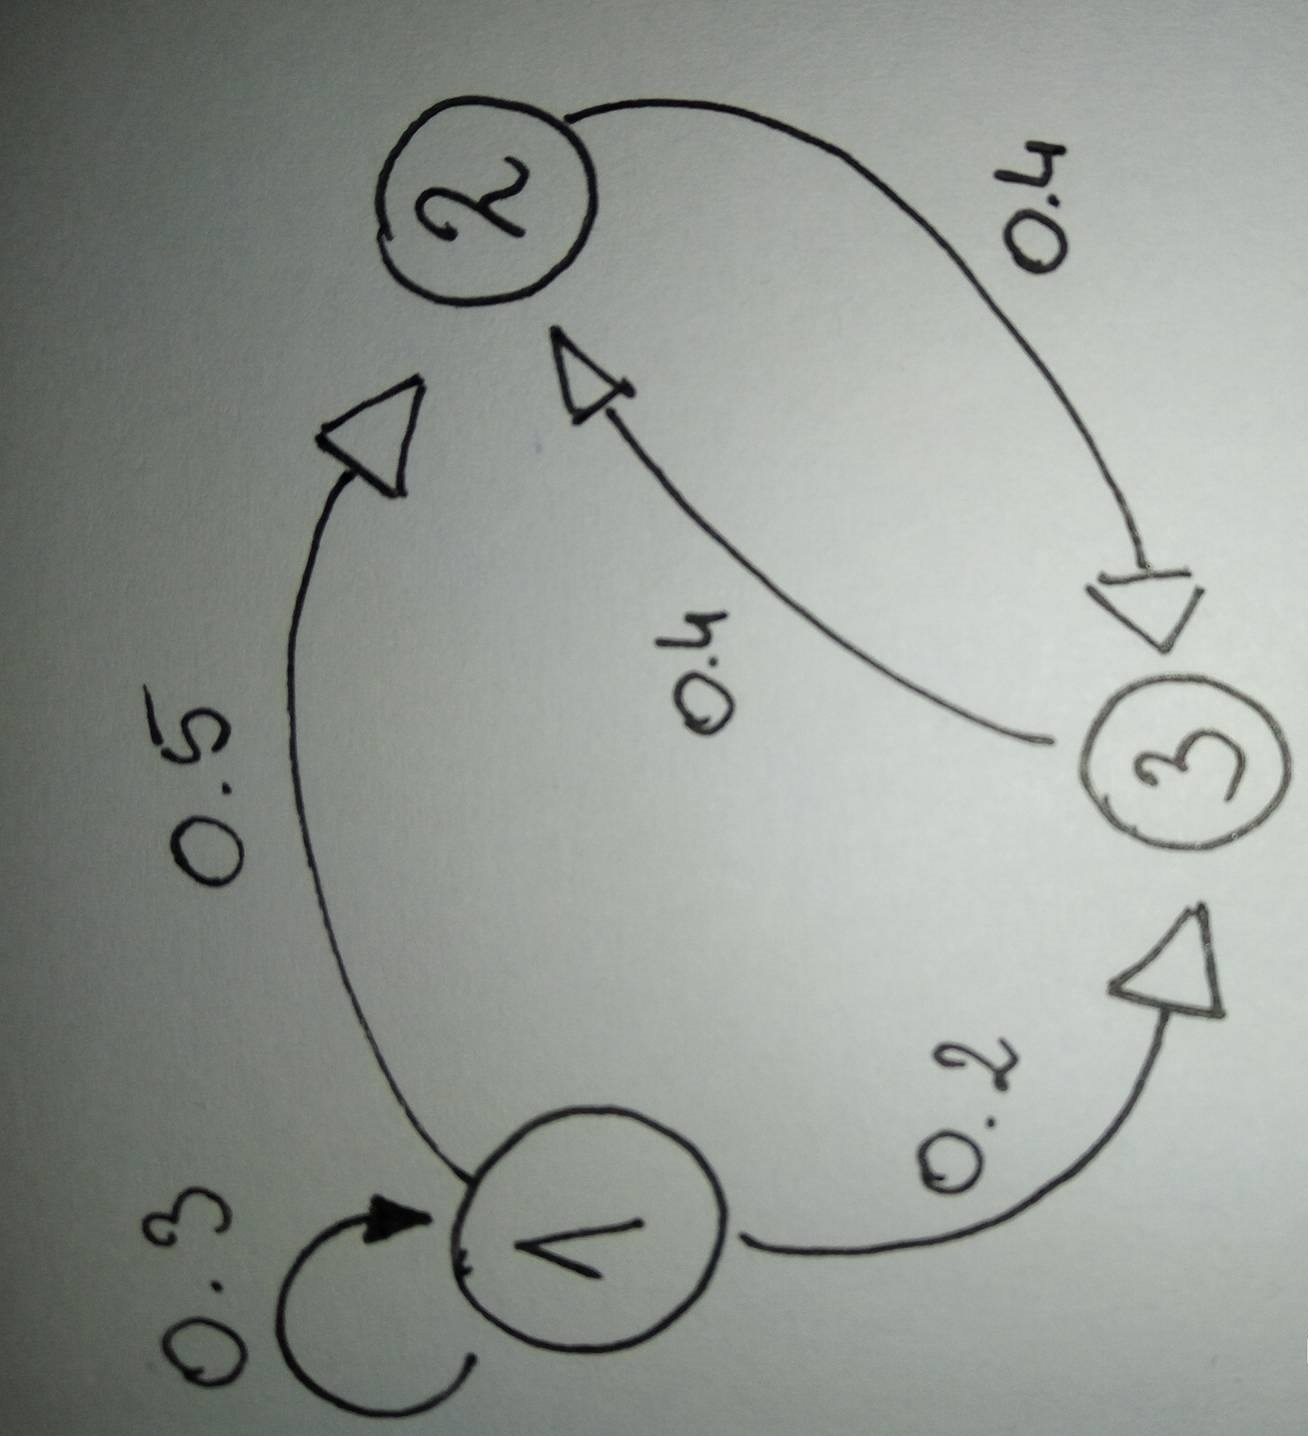
\includegraphics[width=90mm, angle =270]{./tydzien_09/markow.jpg}
\subsection{Zadanie 8}

\begin{center}
\begin{tabular}{ | l | c | c | c | }
\hline  
 \qquad  $Y$ & Y = 0 & Y = 1 & py \\
  $X$ &  &  &  \\
\hline  
 X = 1 & $\frac{1}{6}$ & $\frac{1}{3}$  & $\frac{1}{2}$ \\
\hline  
 X = 2 & $\frac{1}{4}$ & $\frac{1}{4}$ & $\frac{1}{2}$   \\
\hline  
px & $\frac{5}{12}$ & $\frac{7}{12}$  & \\
\hline  
\end{tabular}
\end{center}

$$ E(X) = 1 * \frac{1}{2} + 2 *  \frac{1}{2} = \frac{3}{2}$$
$$ E(Y) = 0 * \frac{5}{12} + 2 *  \frac{7}{12} = \frac{7}{12}$$
$$ E(XY) = 0 * 1 * \frac{1}{6} +  1 * 1 * \frac{1}{3} +  0 * 2 * \frac{1}{4} +  1 * 2 * \frac{1}{4} = \frac{1}{3}* \frac{1}{2} = \frac{5}{6}$$
$$ E(XY^2) = 0^2 * 1 * \frac{1}{6} +  1^2 * 1 * \frac{1}{3} +  0^2 * 2 * \frac{1}{4} +  1^2 * 2 * \frac{1}{4} = \frac{5}{6}$$


$$ E(X^2) = \frac{1}{2} + 2= \frac{5}{2}$$
$$ E(Y^2) = \frac{7}{12}$$

\subsection{Zadanie 9}

$$
P = 
\begin{bmatrix}
    0.3 & 0.5 & 0.2 \\
    0.6 & 0 & 0.4 \\
    0 & 0.4 & 0.6 \\
\end{bmatrix}
$$

$$
\begin{cases}
\begin{bmatrix}
    \pi_{1} & \pi_{2} & \pi_{2}
\end{bmatrix}
P = 
\begin{bmatrix}
    \pi_{1} \\
    \pi_{2} \\
    \pi_{2}
\end{bmatrix} \\
\pi_{1} + \pi_{2} + \pi_{2} = 1
\end{cases}
$$

$$
\begin{cases}
0.3\pi_{1} + 0.6\pi_{2}  = \pi_{1} \\
0.5\pi_{1} + 0.4\pi_{2} = \pi_{2} \\
0.2\pi_{1} + 0.4\pi_{2} + 0.6\pi_{2} = \pi_{3} \\
\pi_{1} + \pi_{2} + \pi_{2} = 1
\end{cases}
$$

$$
\begin{cases}
\pi_{1} = \frac{12}{46} \\
\pi_{2} = \frac{14}{46} \\
\pi_{3} = \frac{20}{46} \\
\end{cases}
$$

\subsection{Zadanie 10}

W - wolny
Z - zajęty
$$
A= \left[ 
        \begin{array}{cc}
         0,8_{z/z} & 0,2_{z/w}\\ 
         0,1_{w/z} & 0,9_{w/w}
         \end{array}
      \right] 
      \qquad$$
      a)\\$$
      \left[ 
        \begin{array}{cc}
         0 & 1
         \end{array}
      \right] \cdot
      \left[ 
        \begin{array}{cc}
         0,8 & 0,2\\ 
         0,1 & 0,9
         \end{array}
      \right] 
      \cdot
      \left[ 
        \begin{array}{cc}
         0,8 & 0,2\\ 
         0,1 & 0,9
         \end{array}
      \right] = \left[ 
        \begin{array}{cc}
         0,17 & 0,83
         \end{array}
      \right] 
      \qquad 
      $$
      b)\\
      $$
      \left[ 
        \begin{array}{cc}
         \pi_1 & \pi_2
         \end{array}
      \right] \cdot
      \left[ 
        \begin{array}{cc}
         0,8 & 0,2\\ 
         0,1 & 0,9
         \end{array}
      \right]  = \left[ 
        \begin{array}{cc}
         \pi_1 & \pi_2
         \end{array}
      \right]$$
\begin{equation}
    \left\{\begin{array}{rcl}
                     0,8\cdot\pi_1+ 0,1\cdot\pi_2 = \pi_1\\
                     0,2\cdot\pi_1+ 0,9\cdot\pi_2 = \pi_2\\
                     \pi_1+ \pi_2 = 1
\end{array}\right.
\end{equation}
Po przekształceniach otrzymujemy: $\pi_1 = \frac{1}{3}, \pi_2 = \frac{2}{3}$



\section{Tydzień 10}
\subsection{Zadanie 1}

$$ E(X) = \sum_{i \in I}^{} = x_i * p_i < \infty $$
$$ I = \{ 1,2,3,4,5,6 \}$$
$$ p= \frac{1}{6}$$
$$ E(X) = \frac{1}{6} * 1 + \frac{1}{6} * 2 + \frac{1}{6} * 3 + \frac{1}{6} * 4 + \frac{1}{6} * 5 + \frac{1}{6} * 6 = 3\frac{1}{4}$$

\subsection{Zadanie 2}

$$ q_{995} = F^{-1}(0,95) = 2 * 0,95 - 1 = 1,9 - 1 = 0,09 $$

\subsection{Zadanie 3}
Medianą jest kwantyl stopnia 1/2, czyli szukamy minimalnego i spełniającego warunek :
$$
 \sum_{j=1}^{i} \left( \frac{5}{6}\right)^{j-1}\frac{1}{6} \ge \frac{1}{2}
$$
dla i = 3 mamy: 
$$
\frac{1}{6} + \frac{5}{36} + \frac{25}{216} < \frac{1}{2}
$$
a dla i = 4 mamy: 
$$
\frac{1}{6} + \frac{5}{36} + \frac{25}{216} + \frac{125}{1296} > \frac{1}{2}
$$
czyli mediana jest równa 4.

\subsection{Zadanie 5}

$$
P = 
\left[
\begin{array}{ccc}
0.7 & 0.3  \\
0.4 & 0.6  
\end{array}
\right]
\qquad
\begin{cases} \pi P = \pi \\ \pi_1 + \pi_2 = 1
\end{cases}
$$

$$
\left[
\begin{array}{cc}
\pi_1 & \pi_2
\end{array}
\right]
\left[
\begin{array}{ccc}
0.7 & 0.3  \\
0.4 & 0.6  
\end{array}
\right]
=
\left[
\begin{array}{cc}
0.7\pi_1 + 0.4\pi_2 & 0.3\pi_1 + 0.6\pi_2
\end{array}
\right]
$$

$$
\begin{cases}
0.7\pi_1 + 0.4\pi_2 = \pi_1 \\
0.3\pi_1 + 0.6\pi_2 = \pi_2 \\
\pi_1 = 1 - \pi_2
\end{cases}
\qquad
\begin{cases}
-0.3\pi_1 + 0.4\pi_2 = 0 \\
0.3\pi_1 - 0.4\pi_2 = 0 \\
\pi_1 = 1 - \pi_2
\end{cases}
$$

$$
-0.3 + 0.3\pi_2 + 0.4\pi_2 = 0
$$
$$
0.7\pi_2 = 0.3
$$

$$
\pi_2 = \frac{0.3}{0.7} = \frac{3}{7}
\qquad
\pi_1 = \frac{4}{7}
$$
Rozkład stacjonarny to:
$$
\left[
\begin{array}{cc}
\pi_1 & \pi_2
\end{array}
\right]
=
\left[
\begin{array}{cc}
\frac{4}{7} & \frac{3}{7}
\end{array}
\right]
$$

\subsection{Zadanie 6}

$ E(X) = \int\limits_{-\infty}^{\infty}xf(x)dx = \int\limits_{0}^{1}x(a\sqrt{x})dx = a\int\limits_{0}^{1}x^{3\over 2}dx = 
\frac{2}{5} a[ x^{5 \over 2}]^{1}_{0} = \frac{2}{5} a  $

\subsection{Zadanie 7}
$$
F(x) = 1 - (\frac{x}{\sigma})^{-\theta}

\text{Obliczmy gęstość, aby wykorzystać ją potem przy obliczaniu wartości oczekiwanej:}
$$
f(x) = F'(x) = \frac{\theta}{\sigma}(\frac{x}{\sigma})^{-\theta-1} = \theta\sigma^{\theta}x^{-\theta-1}
$$
\text{Pierwszy moment:}
$$
\mu_1 = E(X) = \int\limits_{\sigma}^{\infty} xf(x)dx = \theta\sigma^{\theta} \int\limits_{\sigma}^{\infty}x^{-\theta}dx = \theta\sigma^{\theta}\frac{x^{-\theta+1}}{-\theta+1} \right {|} ^{x=\infty}_{x=\sigma} = \frac{\theta\sigma}{\theta-1},\  dla \  \theta > 1
$$
\text{Drugi moment:}
$$
\mu_2 = E(X^2) = \int\limits_{\sigma}^{\infty}x^2f(x)dx = \theta\sigma^{\theta}\int\limits_{\sigma}^{\infty}x{-\theta+1}dx = \frac{\theta\sigma^2}{\theta-2}, \ dla \ \theta>2
$$
$$
\begin{cases} \mu_1 = \frac{\theta\sigma}{\theta-1} = m_1 \\
\mu_2 = \frac{\theta\sigma^2}{\theta-2} = m_2\end{cases}
$$
$$
\hat{\theta} = \sqrt{\frac{m_2}{m_2-m_1^2}}+1
$$
$$
\hat{\sigma} = \frac{m_1(\hat{\theta}-1)}{\hat{\theta}}
$$

\subsection{Zadanie 8}

$L(x,m,\sigma)=\displaystyle\prod\limits_{i=1}^n f_{m,\sigma} (x_i)$ - funkcja niepewności

$$l=ln L(x,m,\sigma)=ln \displaystyle\prod\limits_{i=1}^n f_{m,\sigma} (x_i)=\displaystyle\sum\limits_{i=1}^n ln(f_{m,\sigma} (x_i))$$

$$l(x)=\displaystyle\sum\limits_{i=1}^n ln(\frac{1}{\sqrt{2\pi\sigma^2}}e^{-\frac{(x-m)^2}{2\sigma^2}})=\displaystyle\sum\limits_{i=1}^n ln (\frac{1}{\sqrt{2\pi\sigma^2}})+\displaystyle\sum\limits_{i=1}^n e^{-\frac{(x-m)^2}{2\sigma^2}}=\displaystyle\sum\limits_{i=1}^n ln (\frac{1}{\sqrt{2\pi\sigma^2}})+\displaystyle\sum\limits_{i=1}^n {\frac{(x-m)^2}{\sigma^2}}$$

$${\frac{\theta}{\theta n}}-L(x_i,m_i,\sigma)=\displaystyle\sum\limits_{i=1}^n 2{\frac{(x_i-m)^2}{2\sigma^2}}={\frac{1}{\sigma^2}}(\displaystyle\sum\limits_{i=1}^n x_i-nm)$$

$${\frac{1}{\sigma^2}}(\displaystyle\sum\limits_{i=1}^n x_i-nm)=0 \Leftrightarrow\displaystyle\sum\limits_{i=1}^n x_i-nm=0$$

$$\displaystyle\sum\limits_{i=1}^n x_i=nm$$

$$m={\frac{\displaystyle\sum\limits_{i=1}^n x_i}{n}}$$

\subsection{Zadanie 9}

$$
P = 
\begin{bmatrix}
    0.3 & 0.5 & 0.2 \\
    0.6 & 0 & 0.4 \\
    0 & 0.4 & 0.6 \\
\end{bmatrix}
$$

$$
\begin{cases}
\begin{bmatrix}
    \pi_{1} & \pi_{2} & \pi_{2}
\end{bmatrix}
P = 
\begin{bmatrix}
    \pi_{1} \\
    \pi_{2} \\
    \pi_{2}
\end{bmatrix} \\
\pi_{1} + \pi_{2} + \pi_{2} = 1
\end{cases}
$$

$$
\begin{cases}
0.3\pi_{1} + 0.6\pi_{2}  = \pi_{1} \\
0.5\pi_{1} + 0.4\pi_{2} = \pi_{2} \\
0.2\pi_{1} + 0.4\pi_{2} + 0.6\pi_{2} = \pi_{3} \\
\pi_{1} + \pi_{2} + \pi_{2} = 1
\end{cases}
$$

$$
\begin{cases}
\pi_{1} = \frac{12}{46} \\
\pi_{2} = \frac{14}{46} \\
\pi_{3} = \frac{20}{46} \\
\end{cases}
$$

\subsection{Zadanie 10}

Z warunków zadania wynika, że dysponujemy próbką prostą $x_{1},...,x_{n}$ z rozkładu ciągłego, 
którego gęstość $f$ jest następująca:
$$
f(x) =
\left\{ \begin{array}{ll}
\frac{1}{a} & \text{gdy } 0 \leq x \leq a \\
0 & \text{wpp}
\end{array} \right.
$$
Funkcją wiarygodności jest więc tutaj:
$$
l(a) = f(x_{1}) \cdot ... \cdot f(x_{n})
$$
W związku z tym, jeżeli wszystkie punkty $x_{i}$ leżą w przedziale $(0, a)$, to:
$$
l(a) = \frac{1}{a^{n}}
$$
Zaś w przeciwnym przypadku:
$$
l(a) = 0
$$
Zatem:
$$
l(a) = 
\left\{ \begin{array}{ll}
\frac{1}{a^n} & \text{dla } a \geq max\{x_{1},...,x_{n}\} \\
0 & \text{dla } 0 < a < max\{x_{1},...,x_{n}\}
\end{array} \right.
$$
W nietrywialnym przypadku, czyli gdy $max\{x_{1},...,x_{n}\} > 0$ funkcja ta jest dobrze określona,
lecz nie jest ciągła w punkcie $ a = max\{x_{1},...,x_{n}\}$. \\
Jednak widać, że akurat w tym punkcie funkcja $l$ przyjmuje wartość największą. \\
Tak więc estymatorem największej wiarygodności parametru $a$ jest:
$$
\hat{a} = max\{x_{1},...,x_{n}\}
$$




\end{document}
